\begin{figure*}[t!]
	\centering
\resizebox{1.\linewidth}{!}{
	\renewcommand{\arraystretch}{0.5}
	\begin{tabular}{@{}c@{\hskip .05cm}c@{\hskip .05cm}c@{\hskip .05cm}c@{\hskip .05cm}c@{\hskip .05cm}c@{}}
		\centering
            &
		{\small Input $t_0$}&
		{\small Tracked $t_0$}&
		{\small Tracked $t_1$}&
		{\small Tracked $t_2$}&
		{\small Tracked $t_3$}\\

            \rotatebox[origin=c]{90}{{\footnotesize	Highway}}&
		\raisebox{-0.5\height}{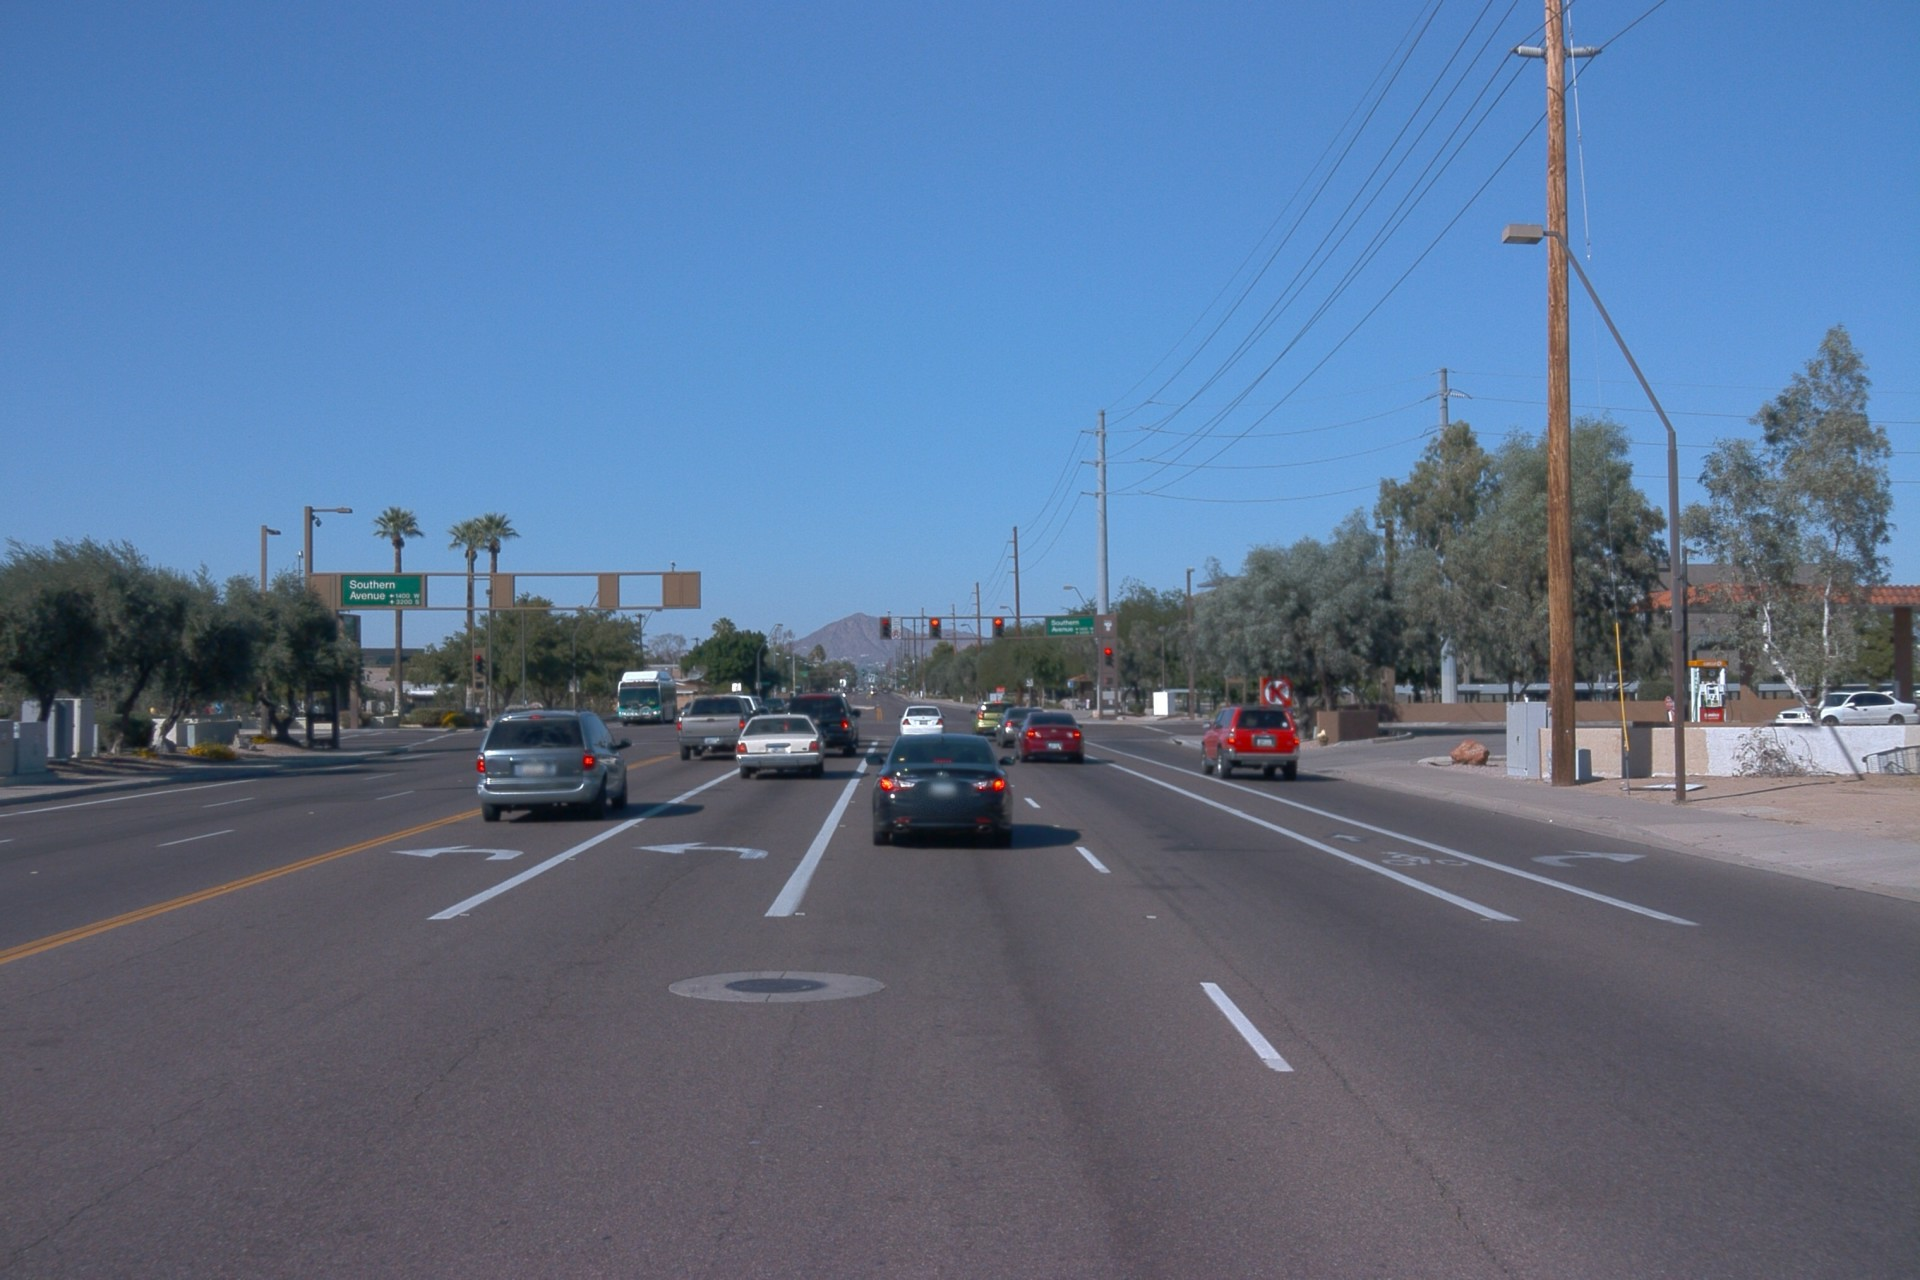
\includegraphics[width=.32\columnwidth, trim={0cm 0cm 0cm 0cm},clip]{fig/waymo_main/scene1/waymo_s50_f45.png}}&
		\raisebox{-0.5\height}{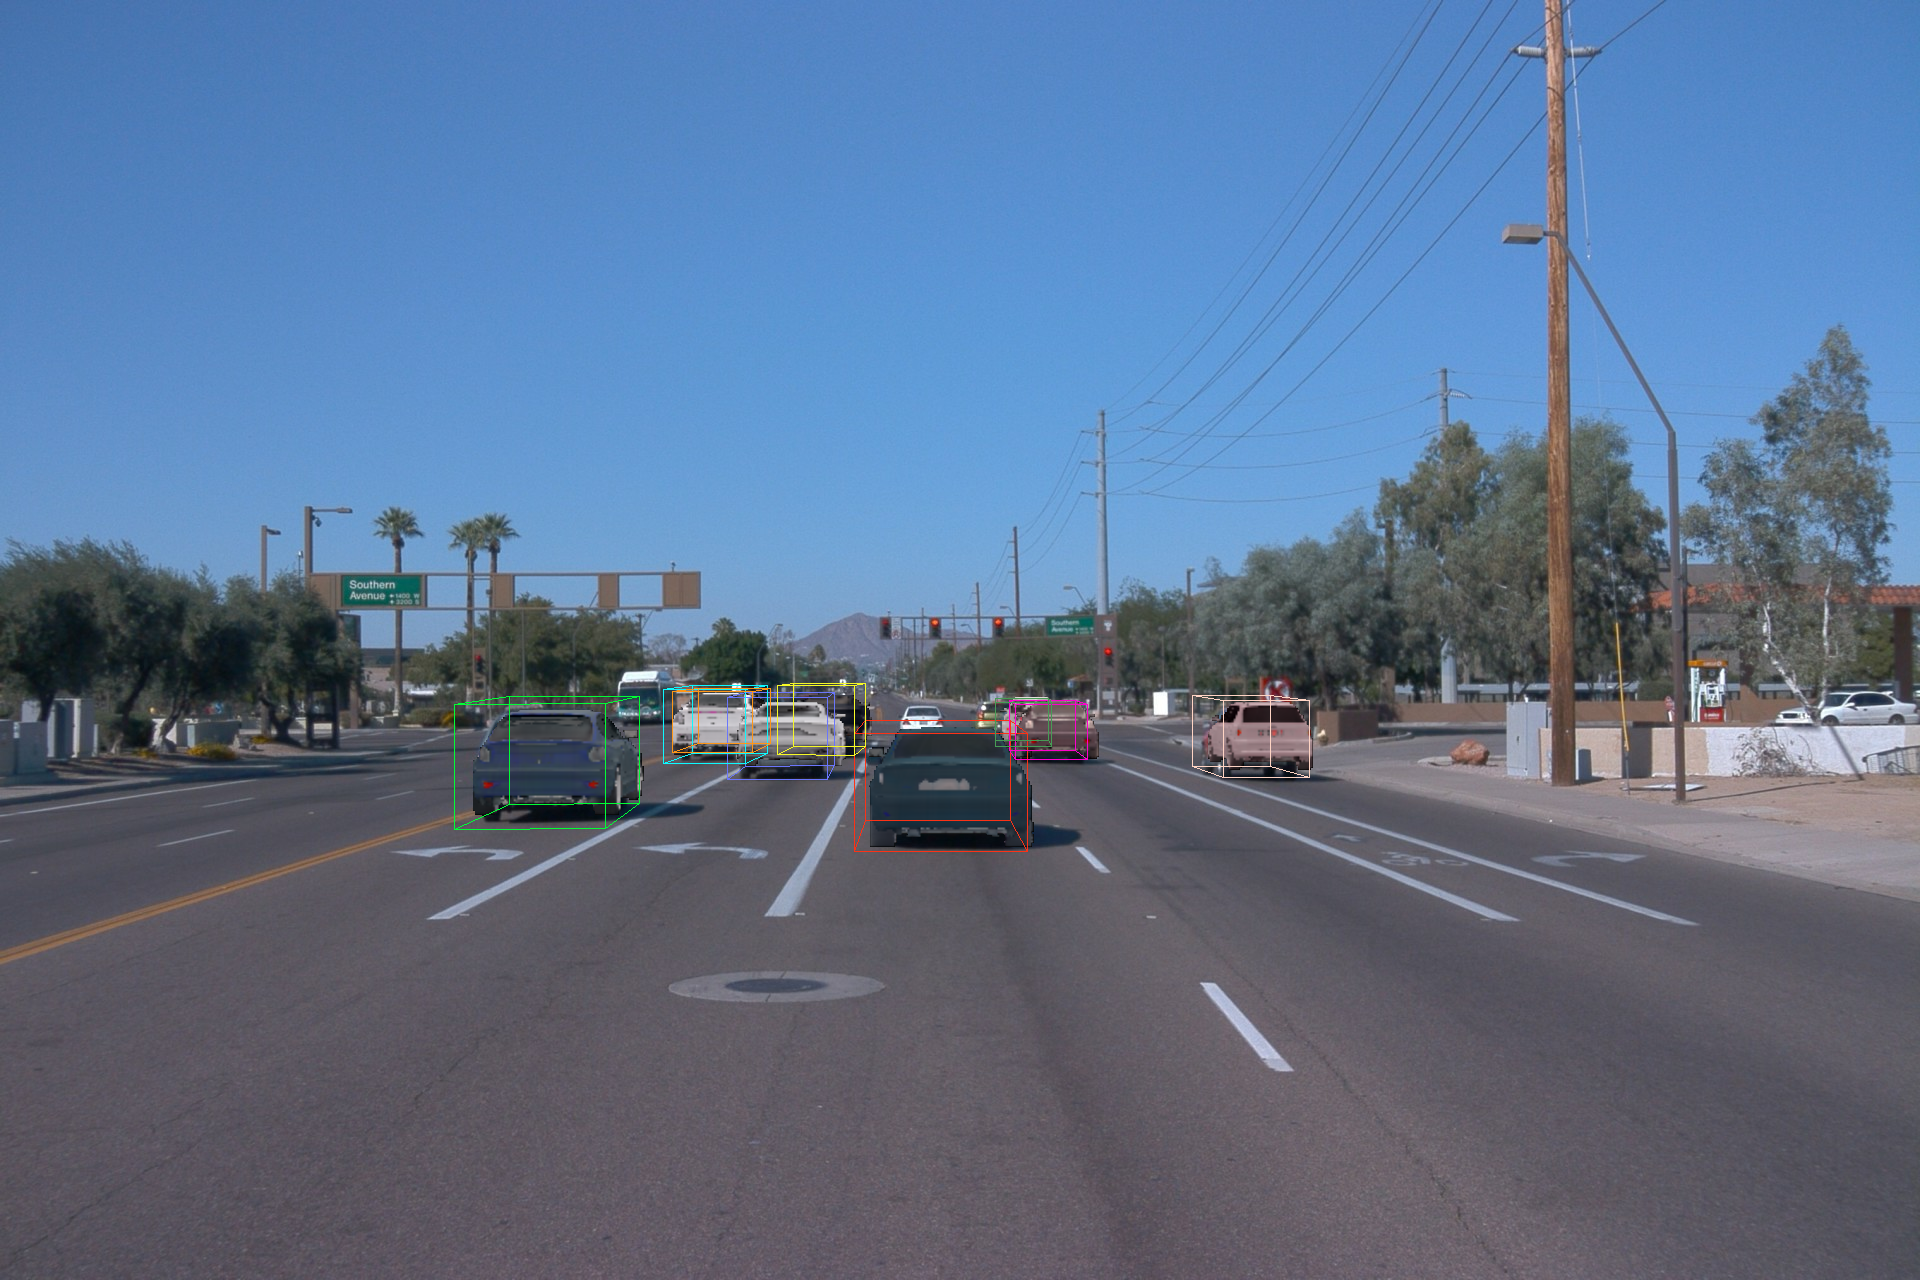
\includegraphics[width=.32\columnwidth, trim={0cm 0cm 0cm 0cm},clip]{fig/waymo_main/scene1/waymo_s50_f45_bbox.png}}&
		\raisebox{-0.5\height}{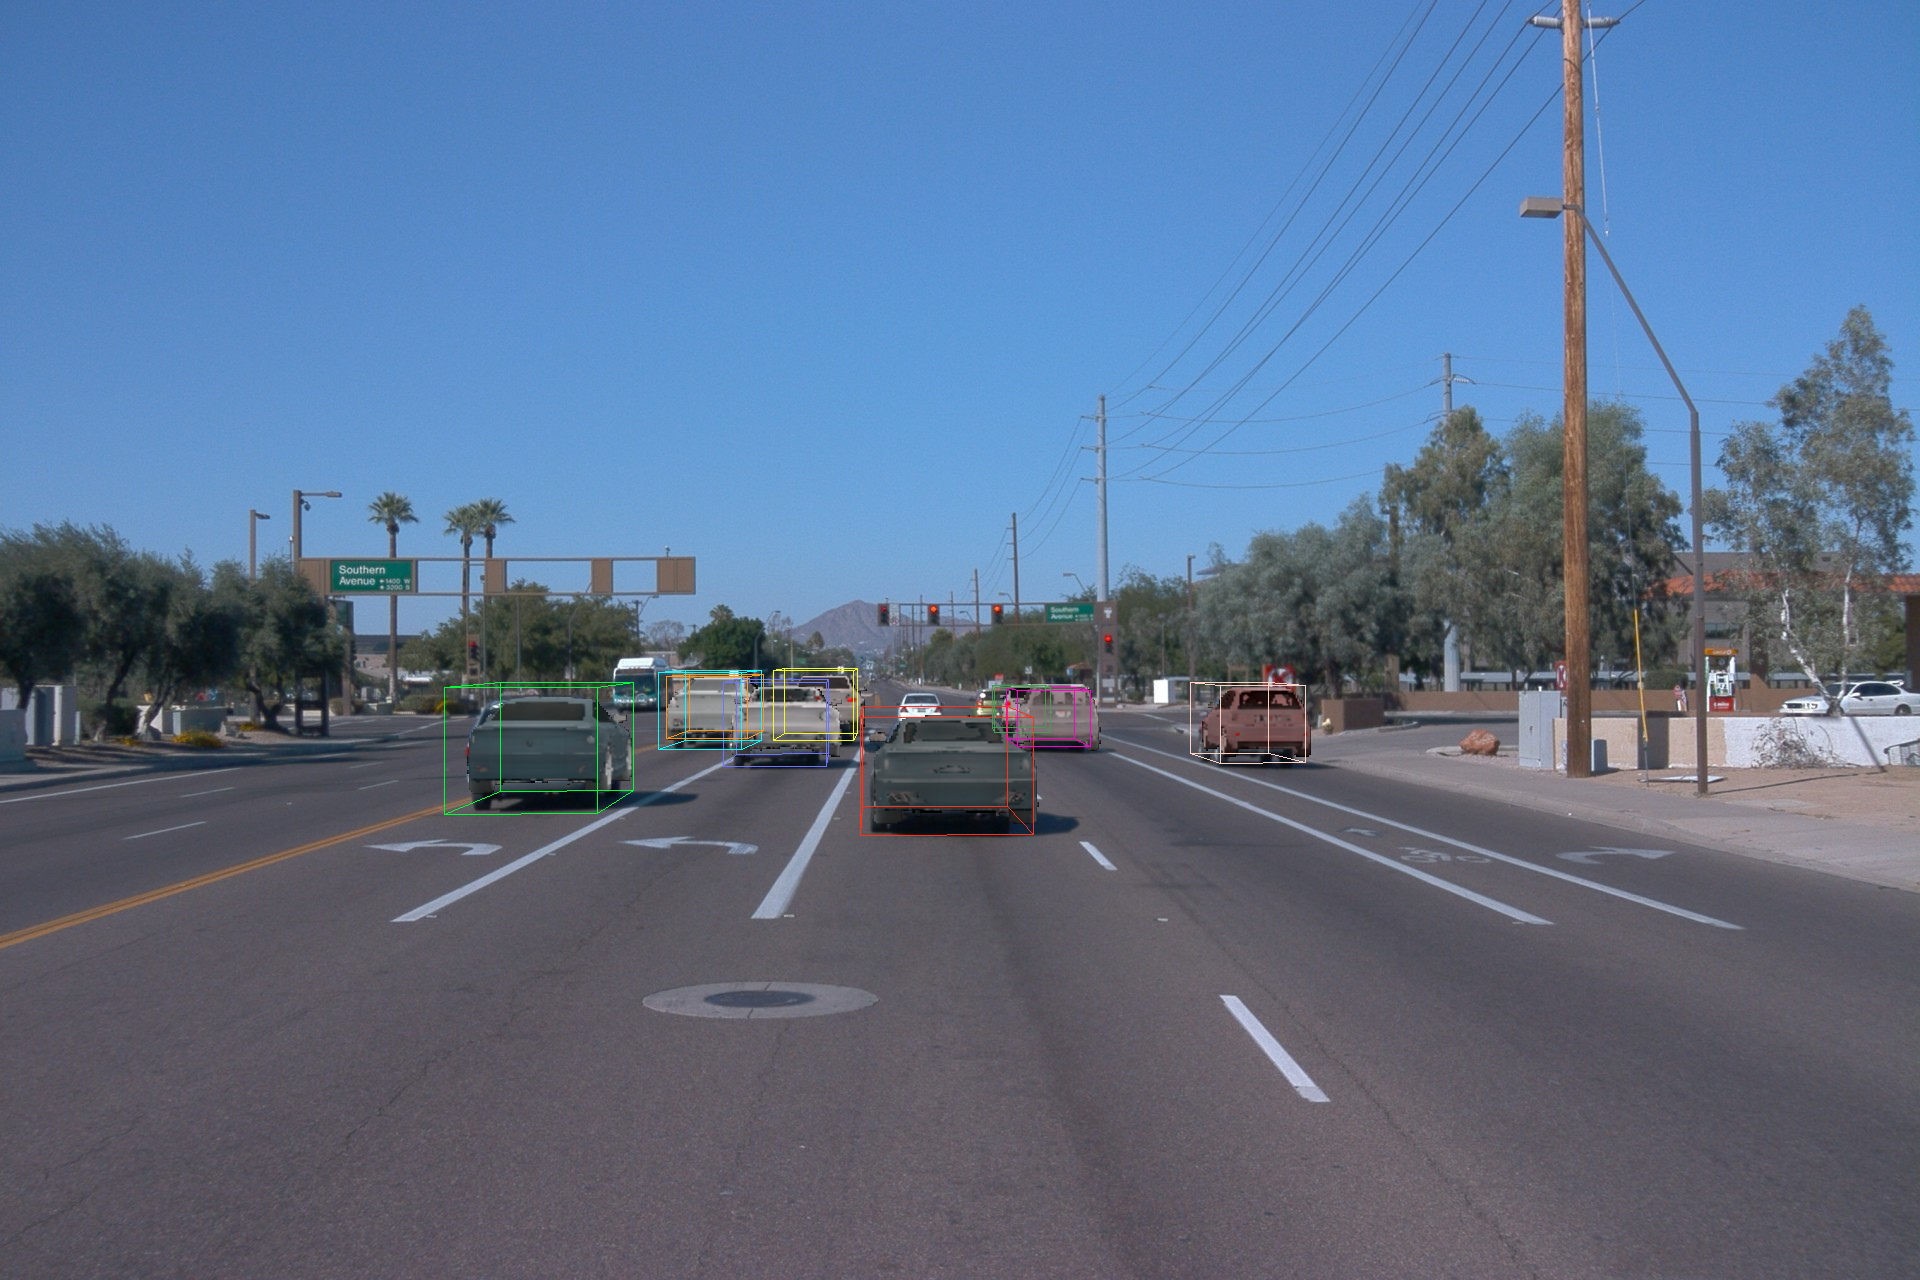
\includegraphics[width=.32\columnwidth, trim={0cm 0cm 0cm 0cm},clip]{fig/waymo_main/scene1/waymo_s50_f46_bbox.png}}&
		\raisebox{-0.5\height}{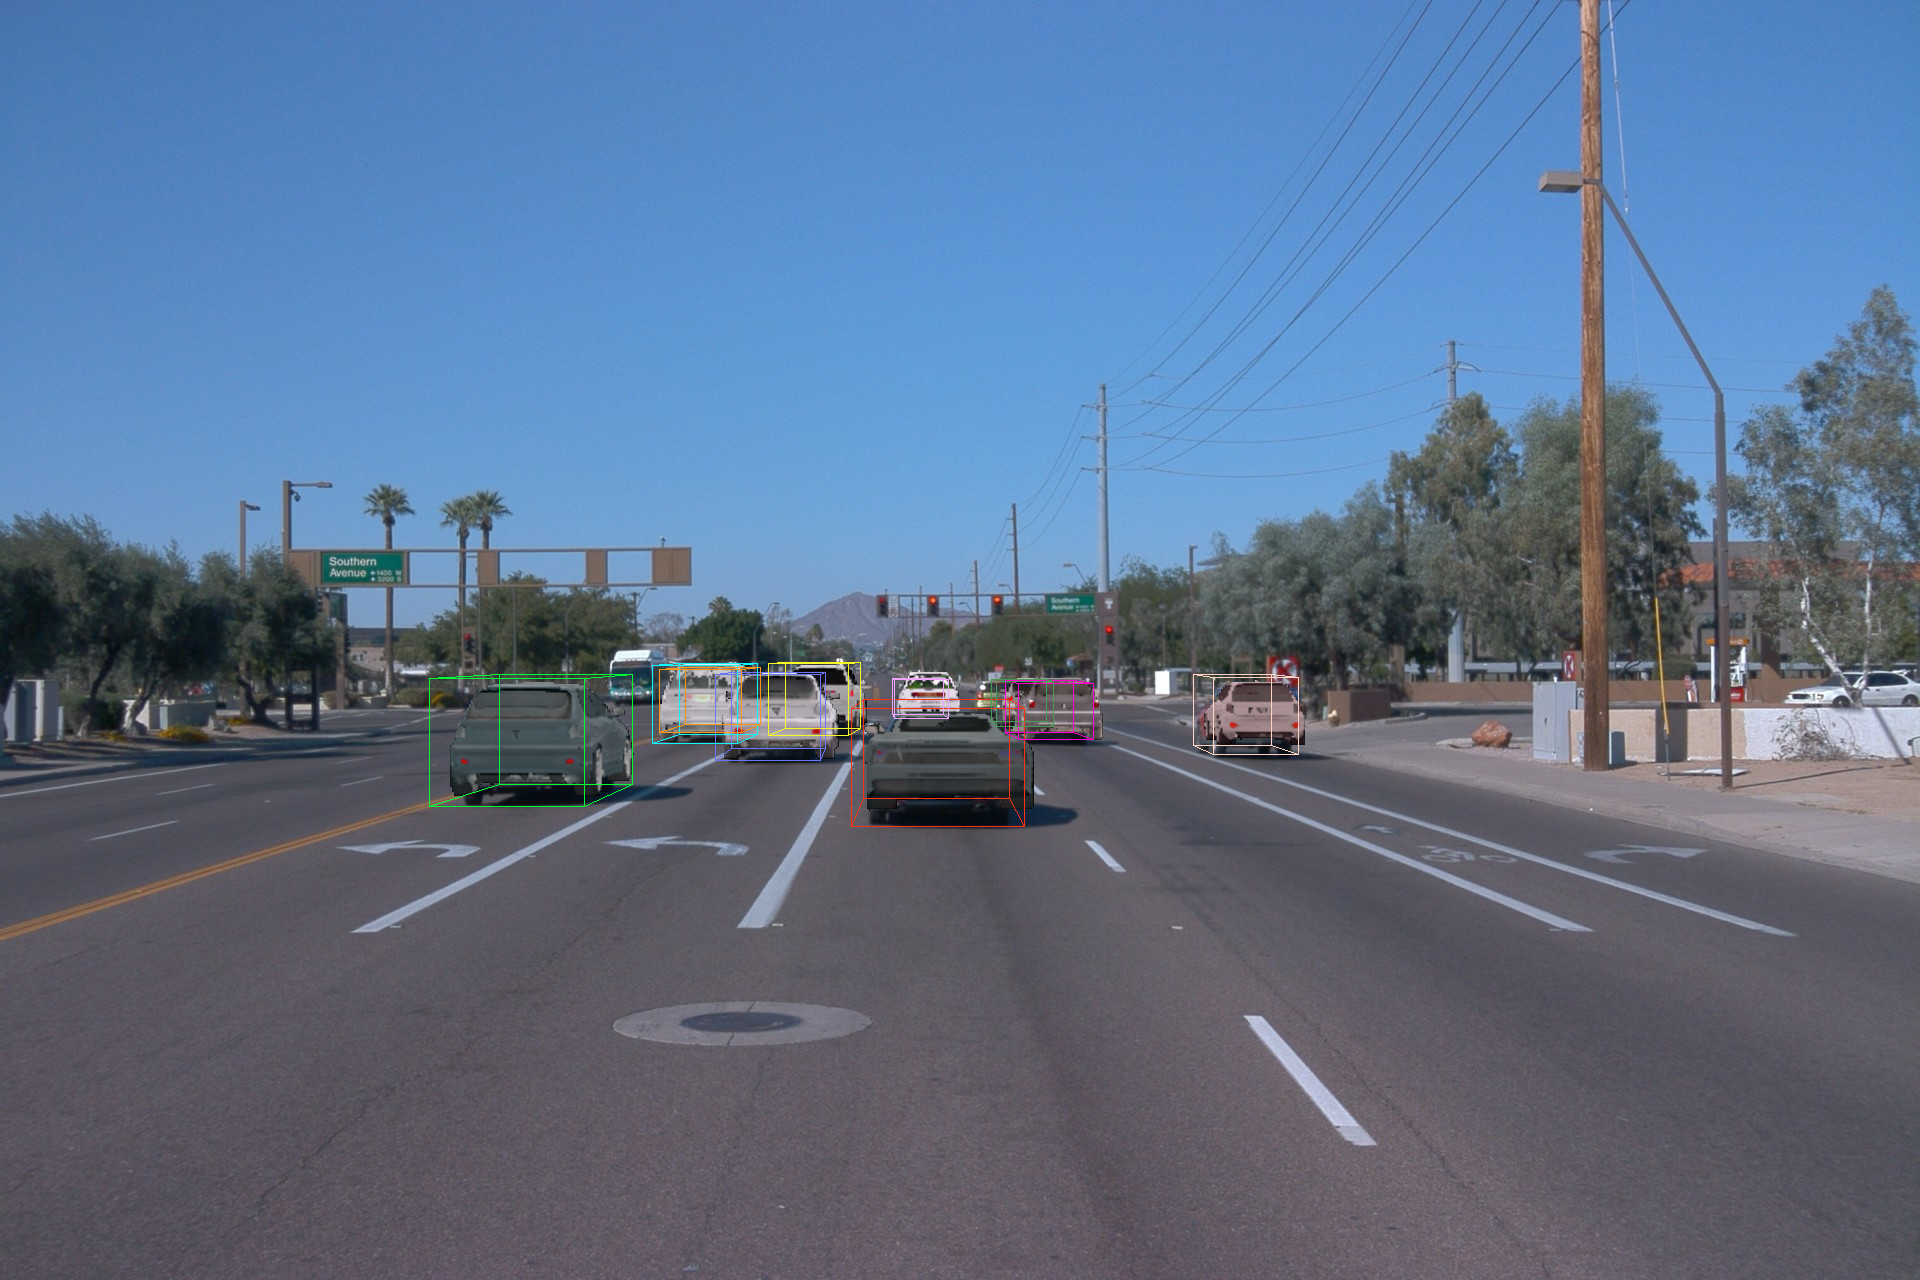
\includegraphics[width=.32\columnwidth, trim={0cm 0cm 0cm 0cm},clip]{fig/waymo_main/scene1/waymo_s50_f47_bbox.png}}&
		\raisebox{-0.5\height}{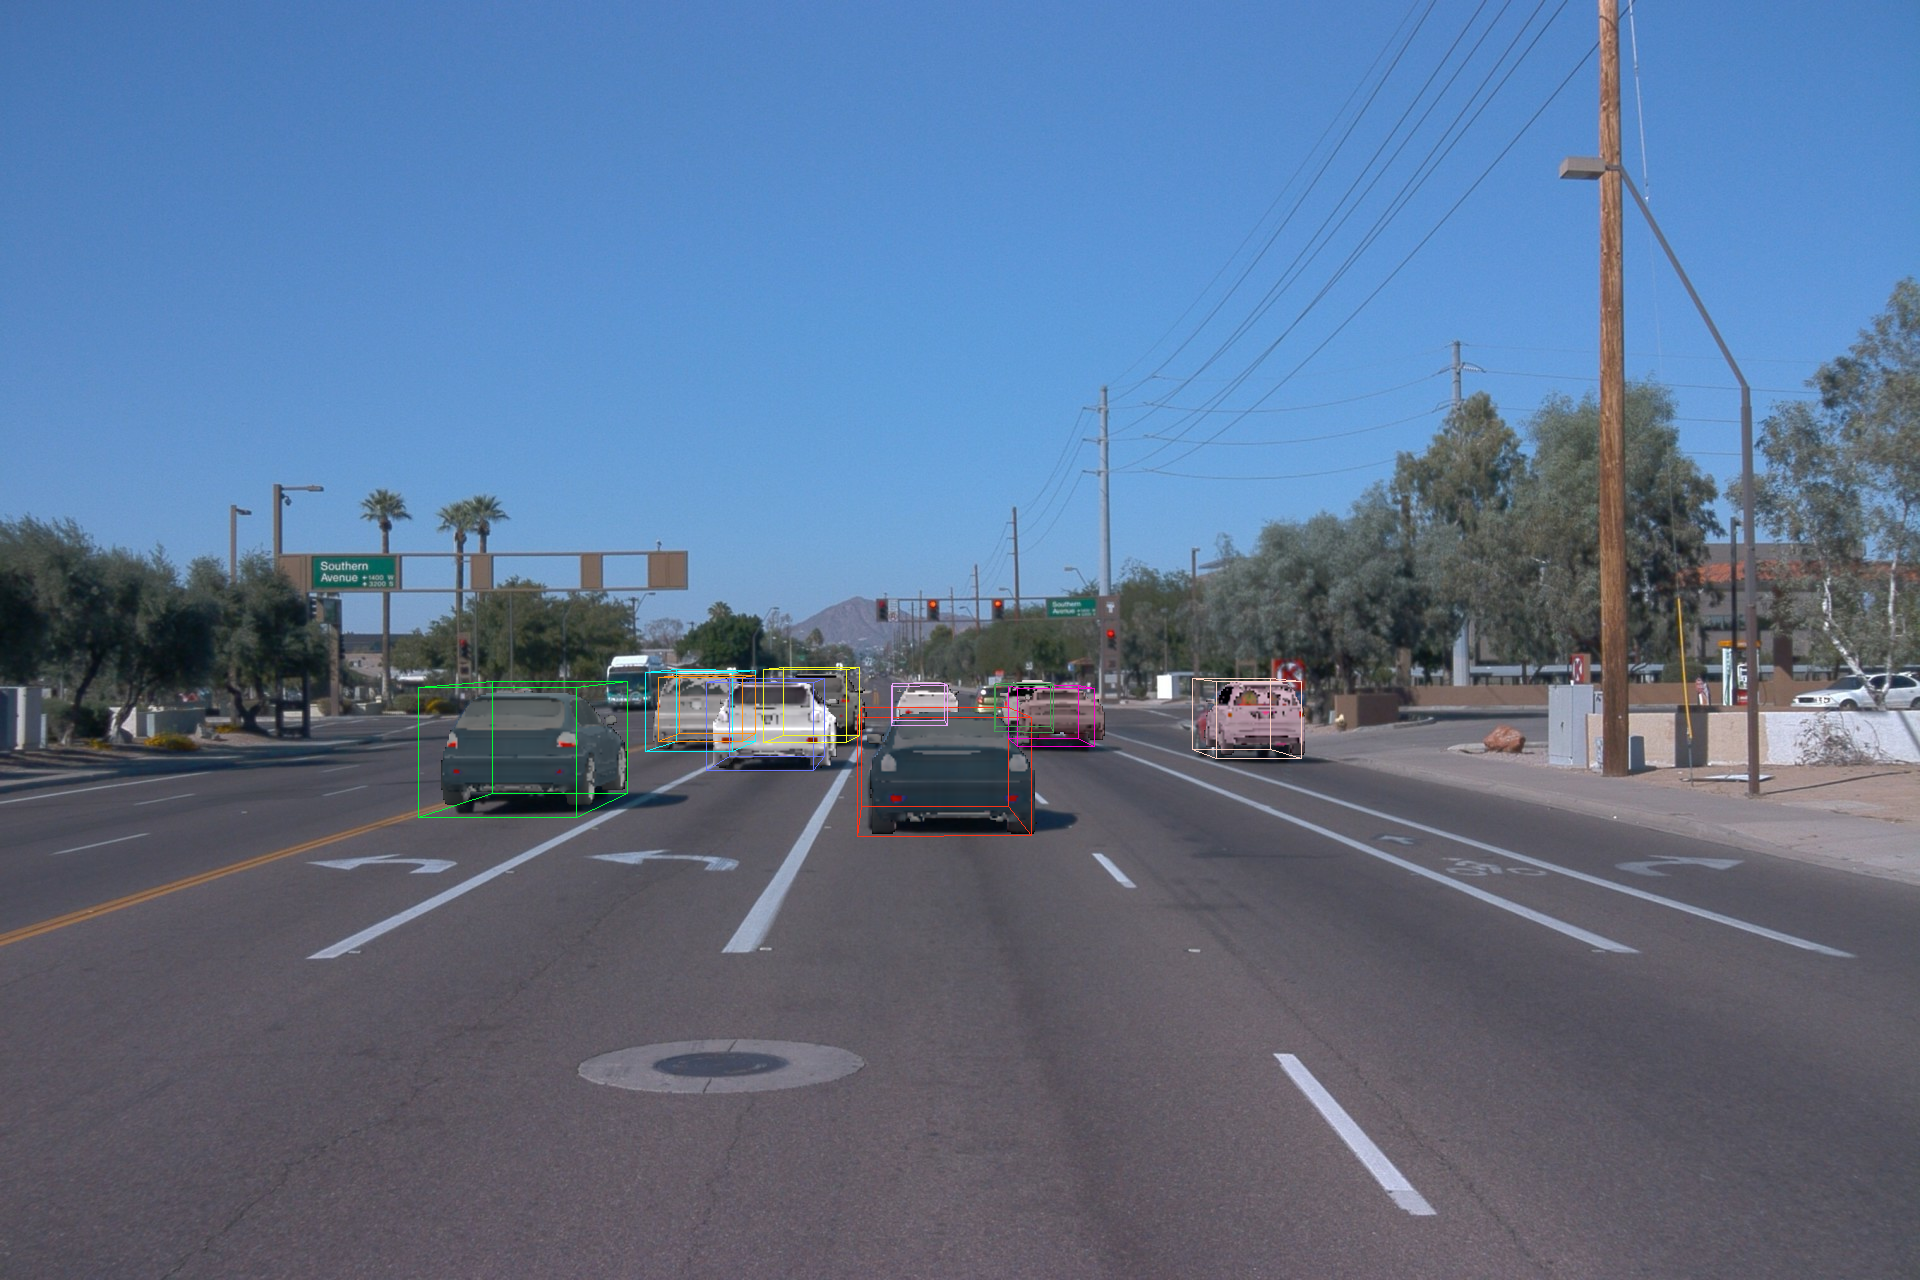
\includegraphics[width=.32\columnwidth, trim={0cm 0cm 0cm 0cm},clip]{fig/waymo_main/scene1/waymo_s50_f48_bbox.png}}\\[1.3cm]

            \rotatebox[origin=c]{90}{{\footnotesize	Urban}}&
		\raisebox{-0.5\height}{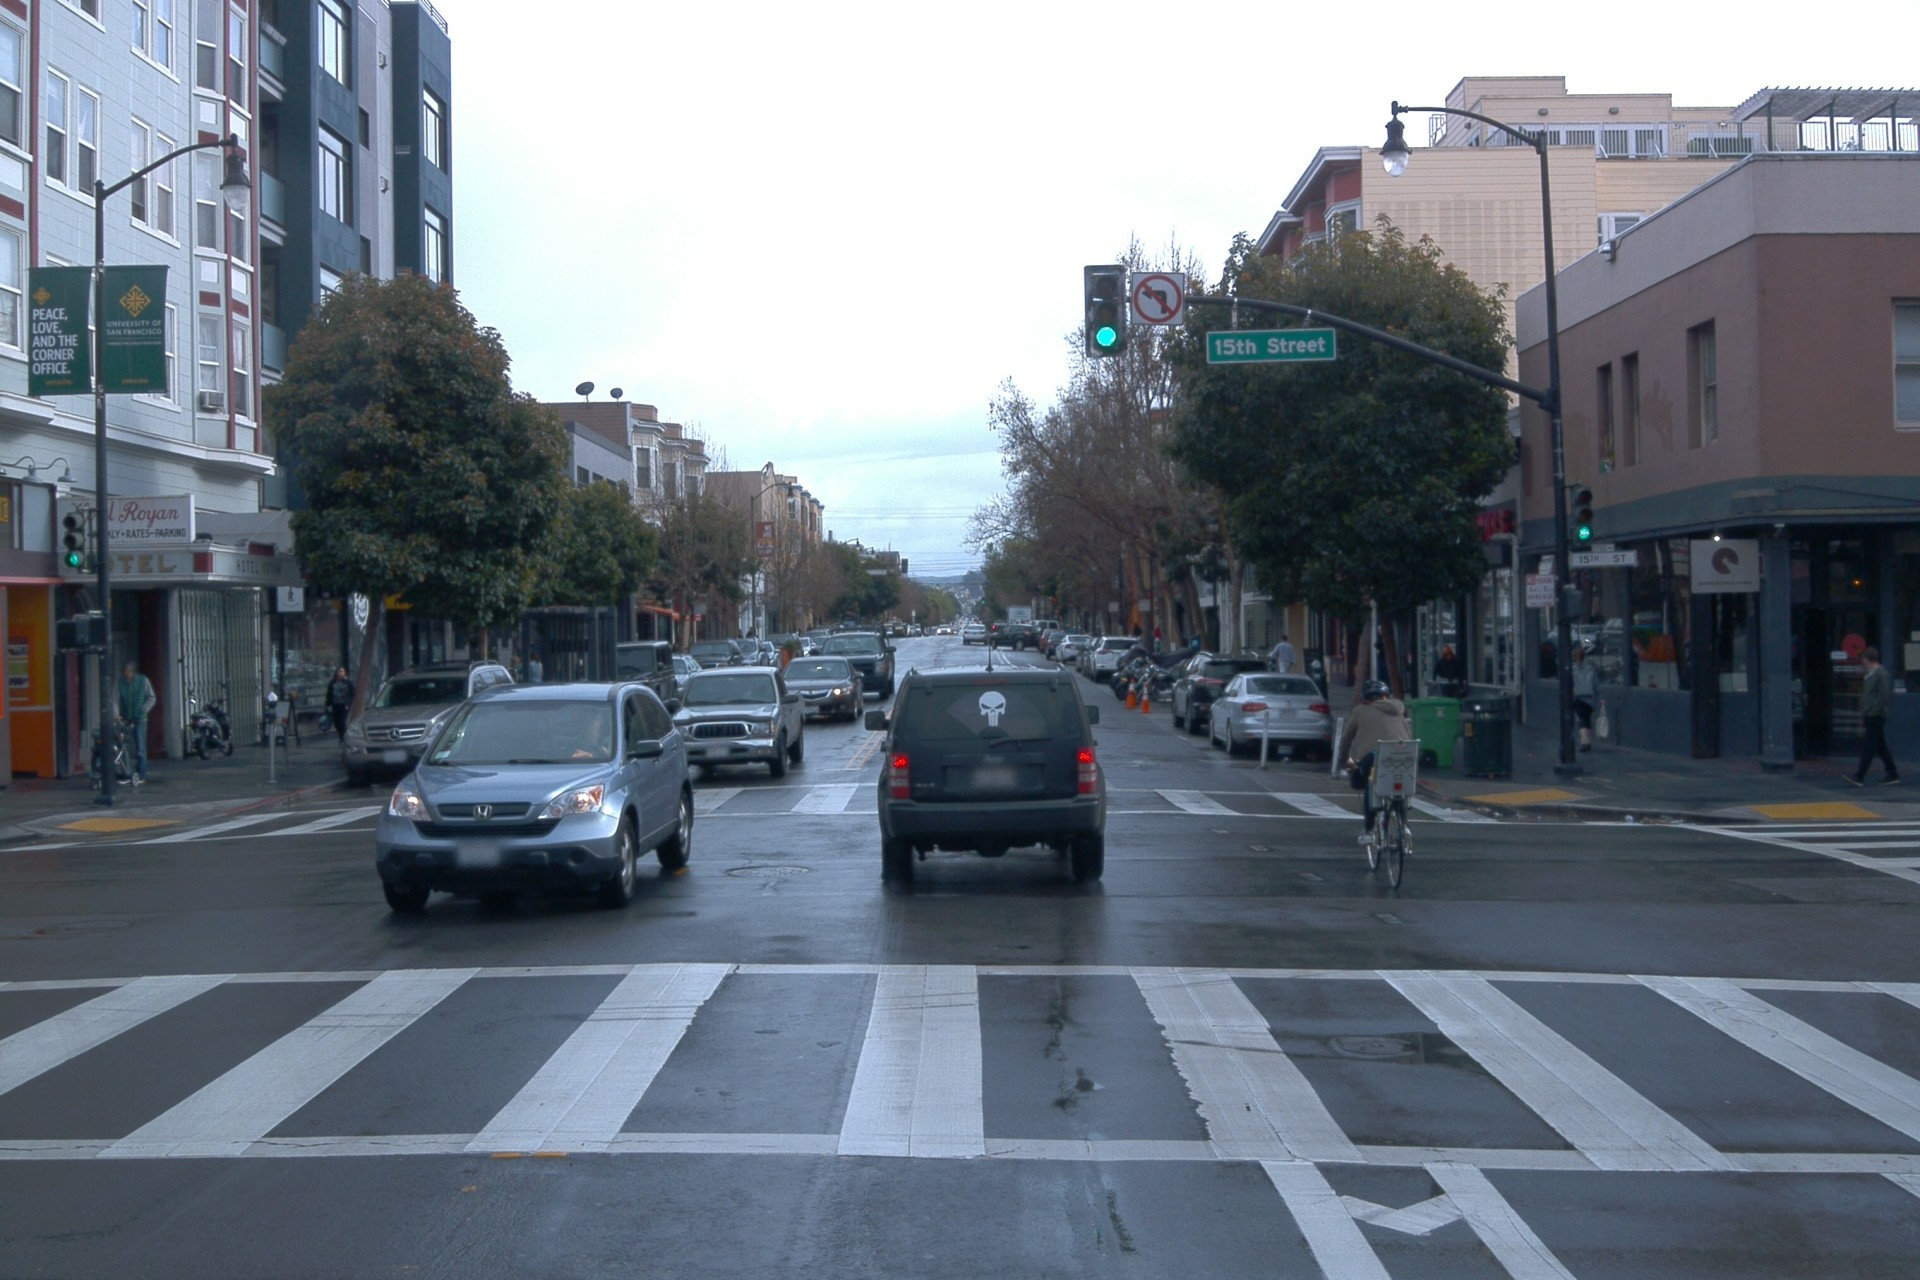
\includegraphics[width=.32\columnwidth, trim={0cm 0cm 0cm 0cm},clip]{fig/waymo_main/scene2/waymo_44_38_gt.png}}&
		\raisebox{-0.5\height}{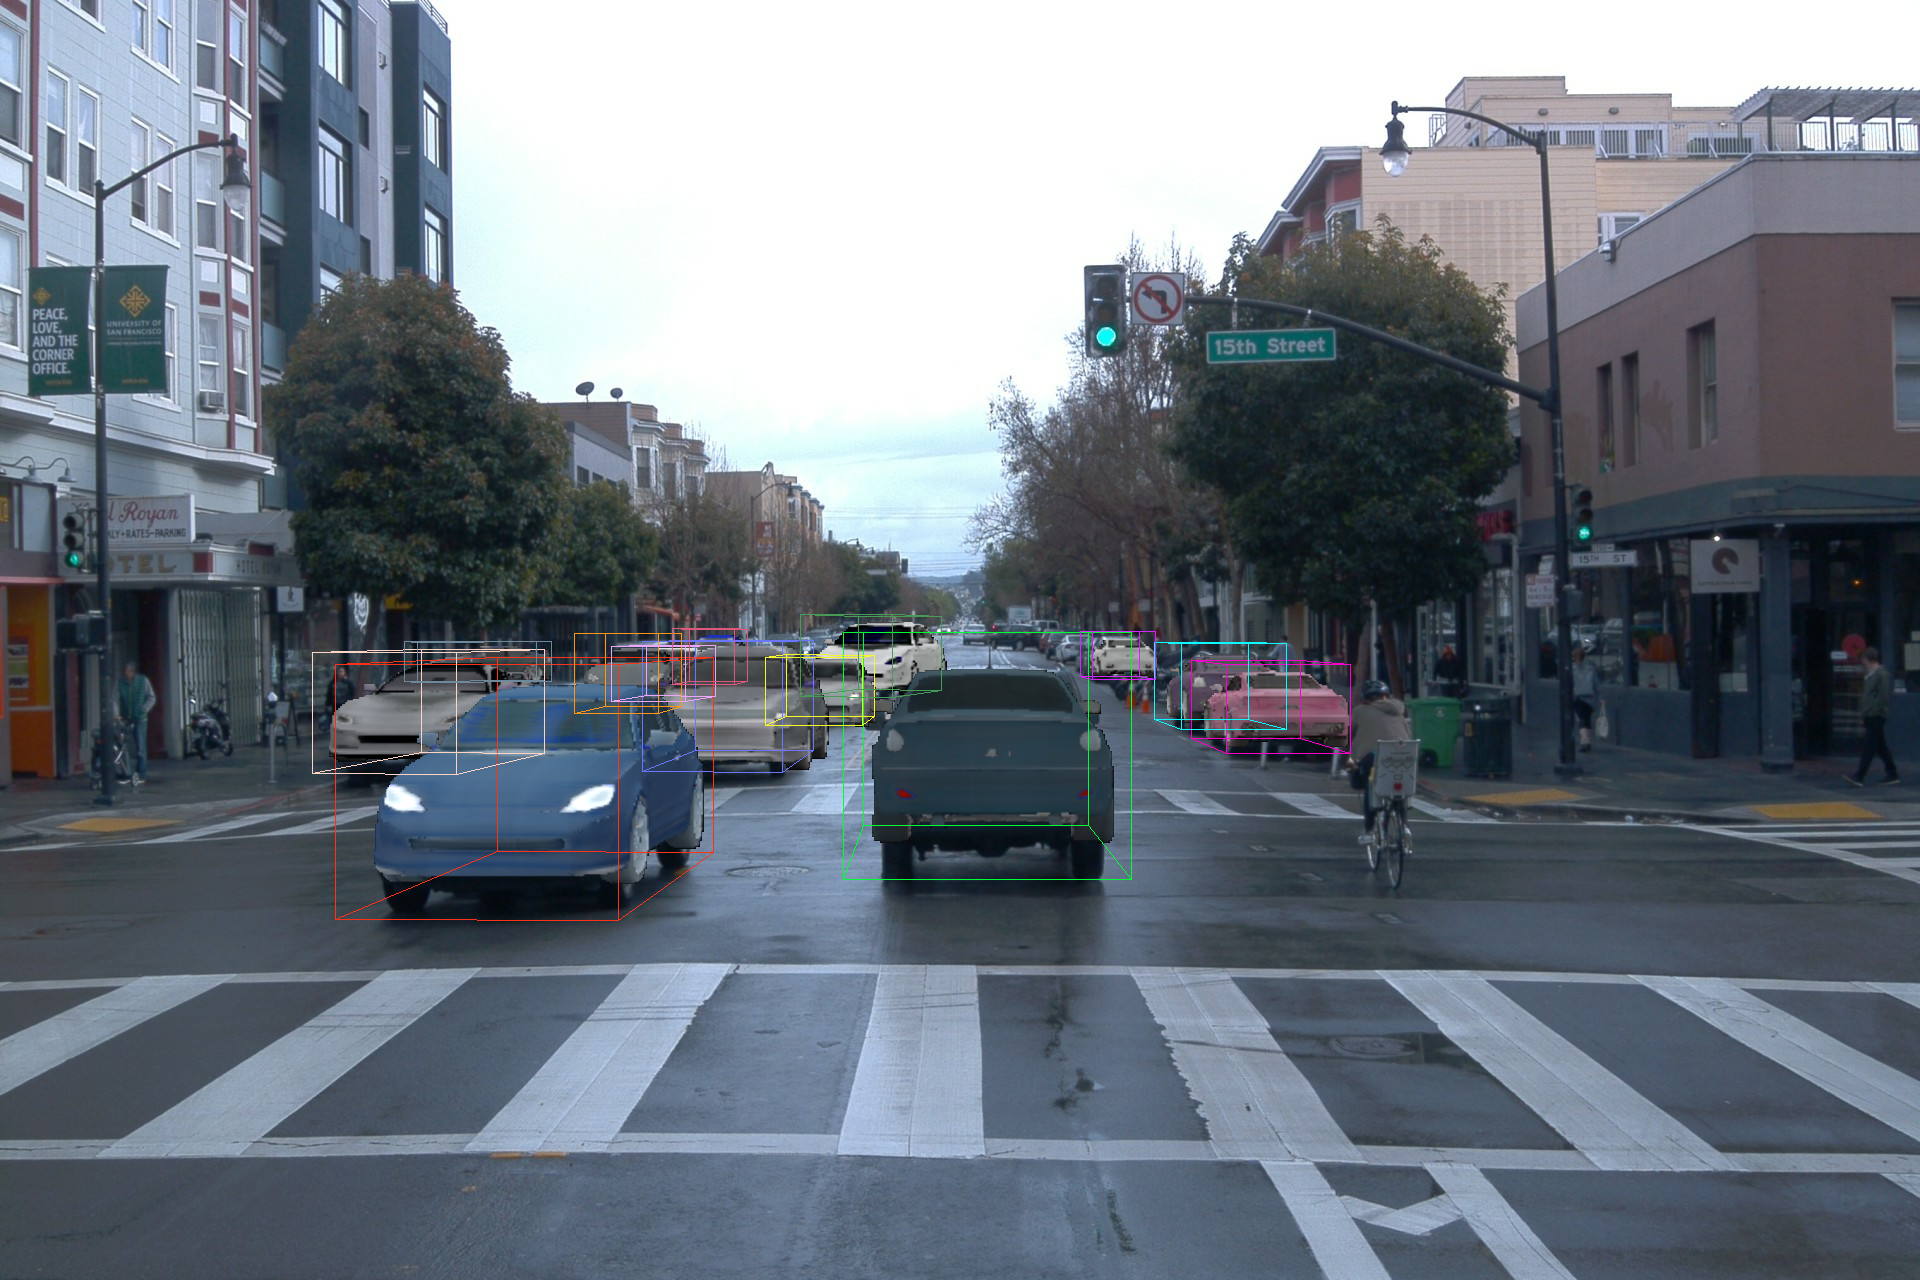
\includegraphics[width=.32\columnwidth, trim={0cm 0cm 0cm 0cm},clip]{fig/waymo_main/scene2/waymo_44_38_bbox.png}}&
		\raisebox{-0.5\height}{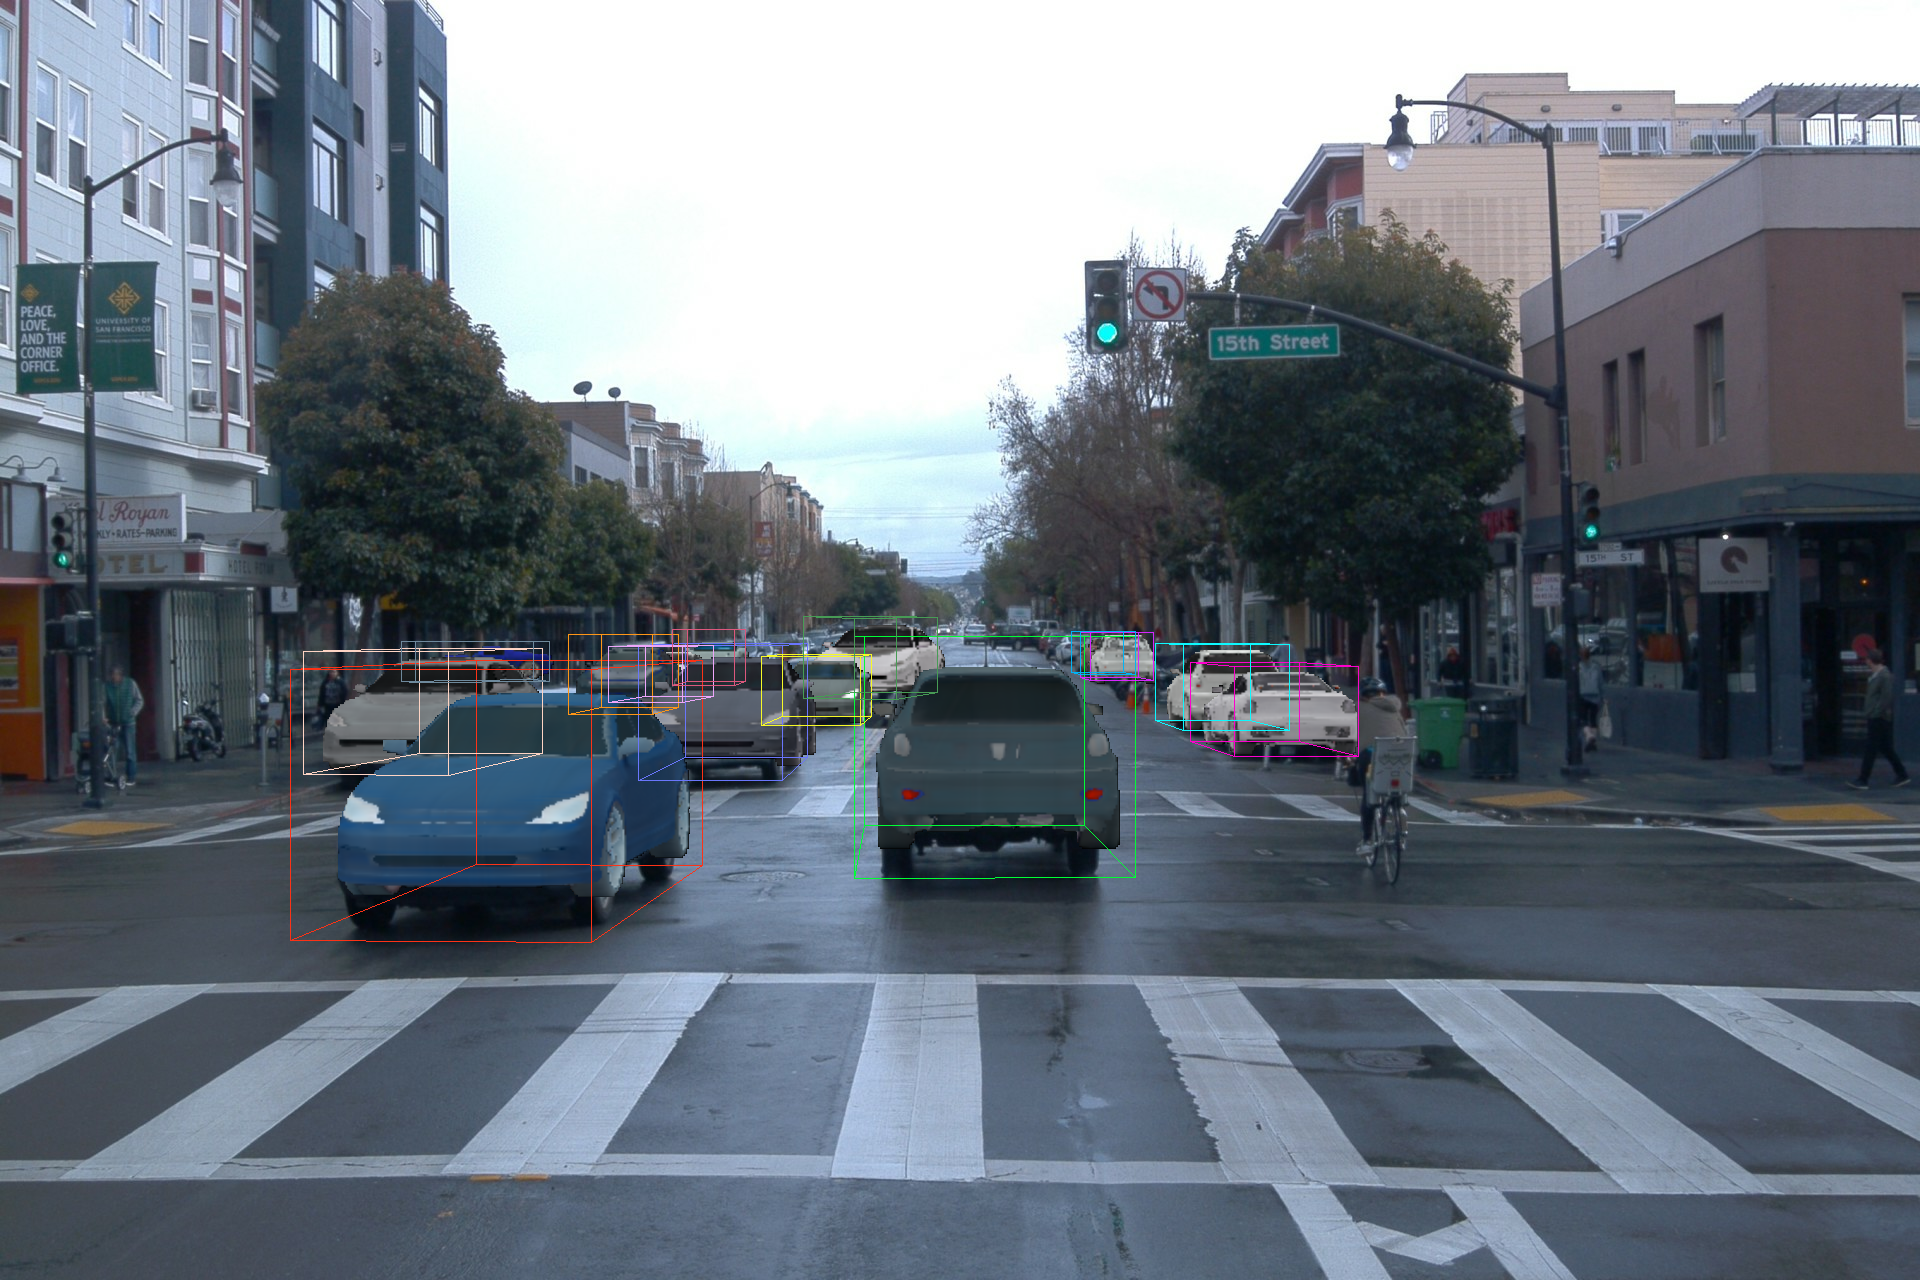
\includegraphics[width=.32\columnwidth, trim={0cm 0cm 0cm 0cm},clip]{fig/waymo_main/scene2/waymo_44_39_bbox.png}}&
		\raisebox{-0.5\height}{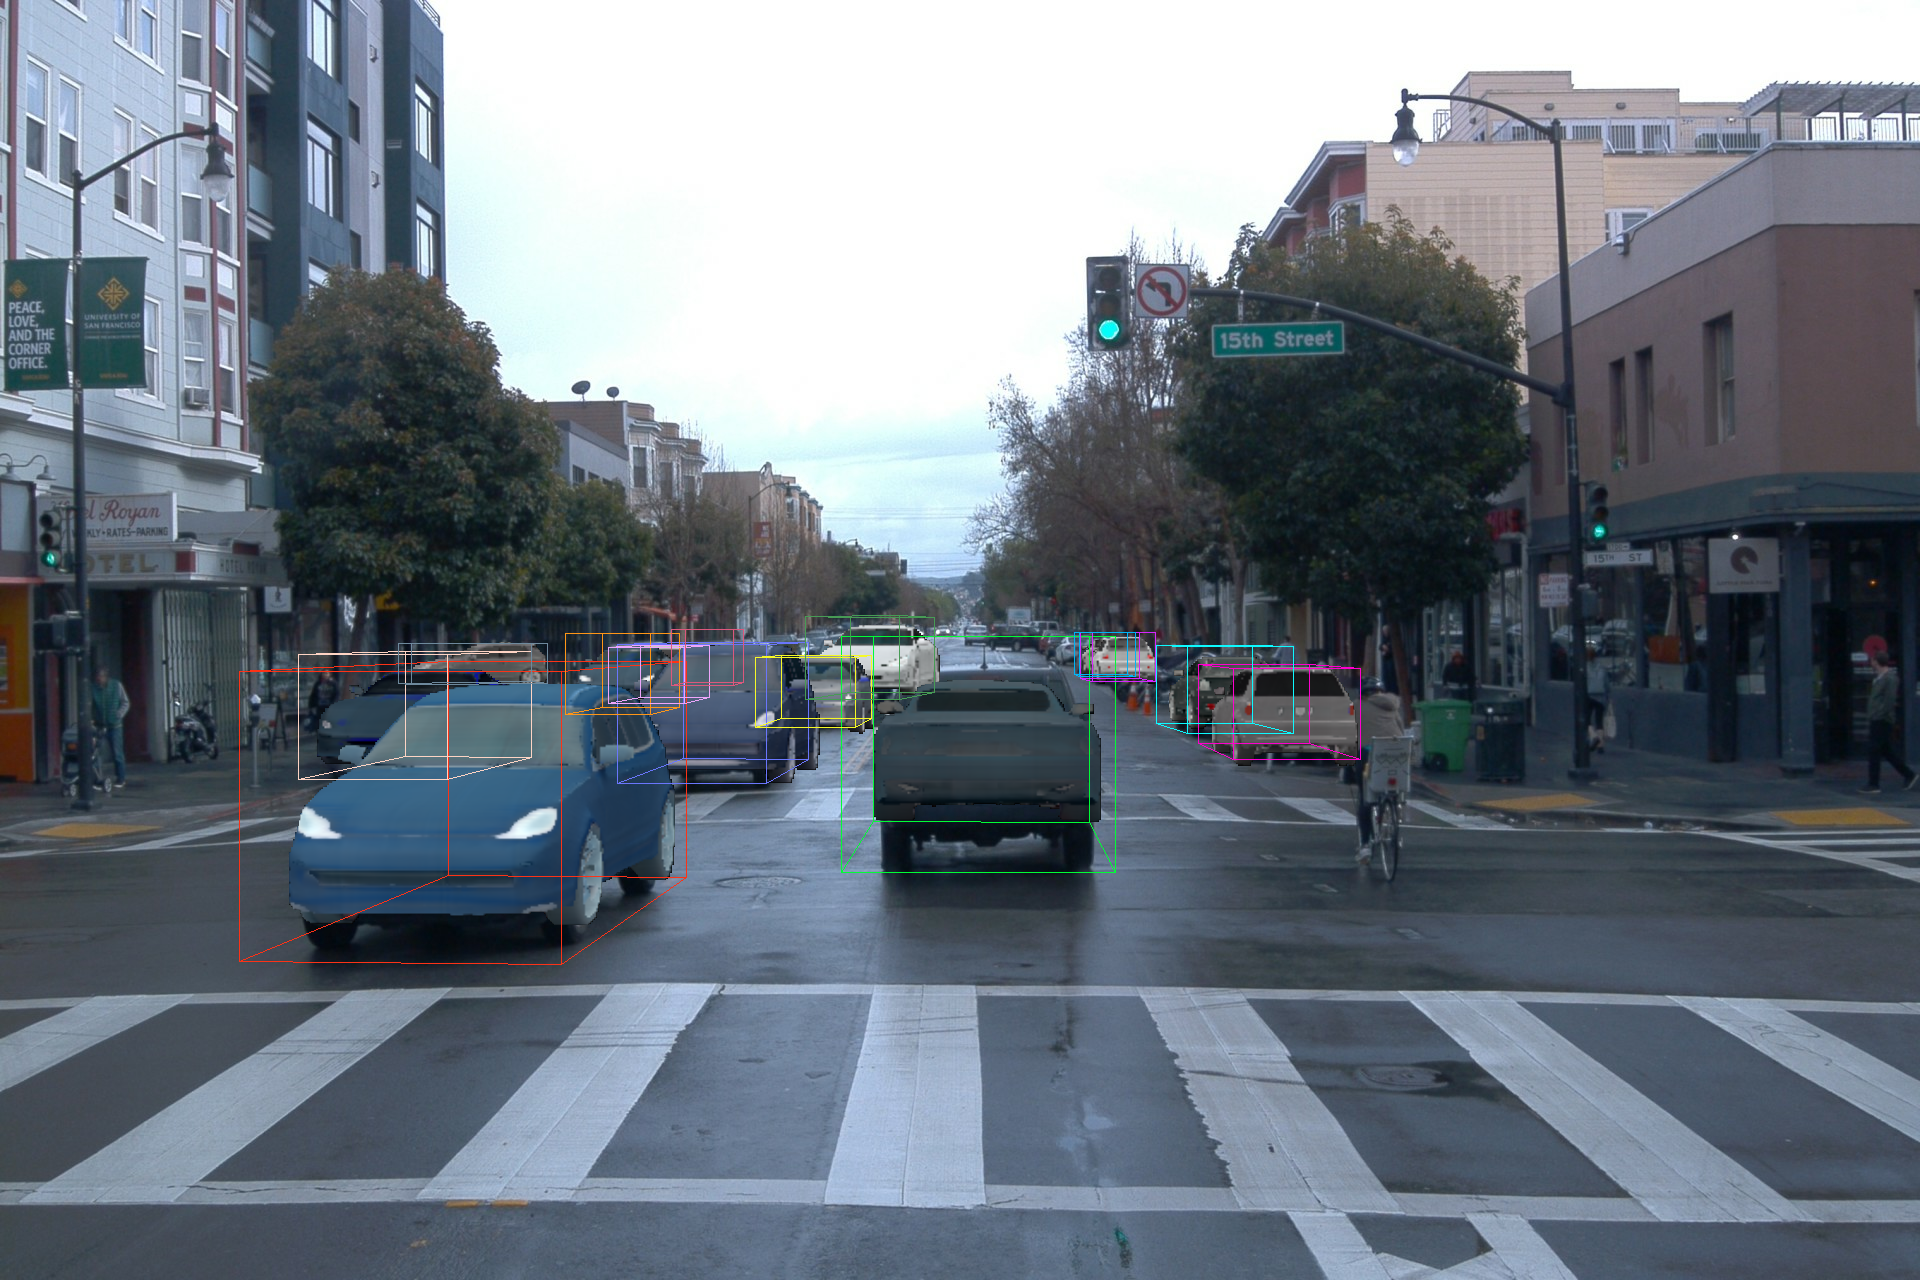
\includegraphics[width=.32\columnwidth, trim={0cm 0cm 0cm 0cm},clip]{fig/waymo_main/scene2/waymo_44_40_bbox.png}}&
		\raisebox{-0.5\height}{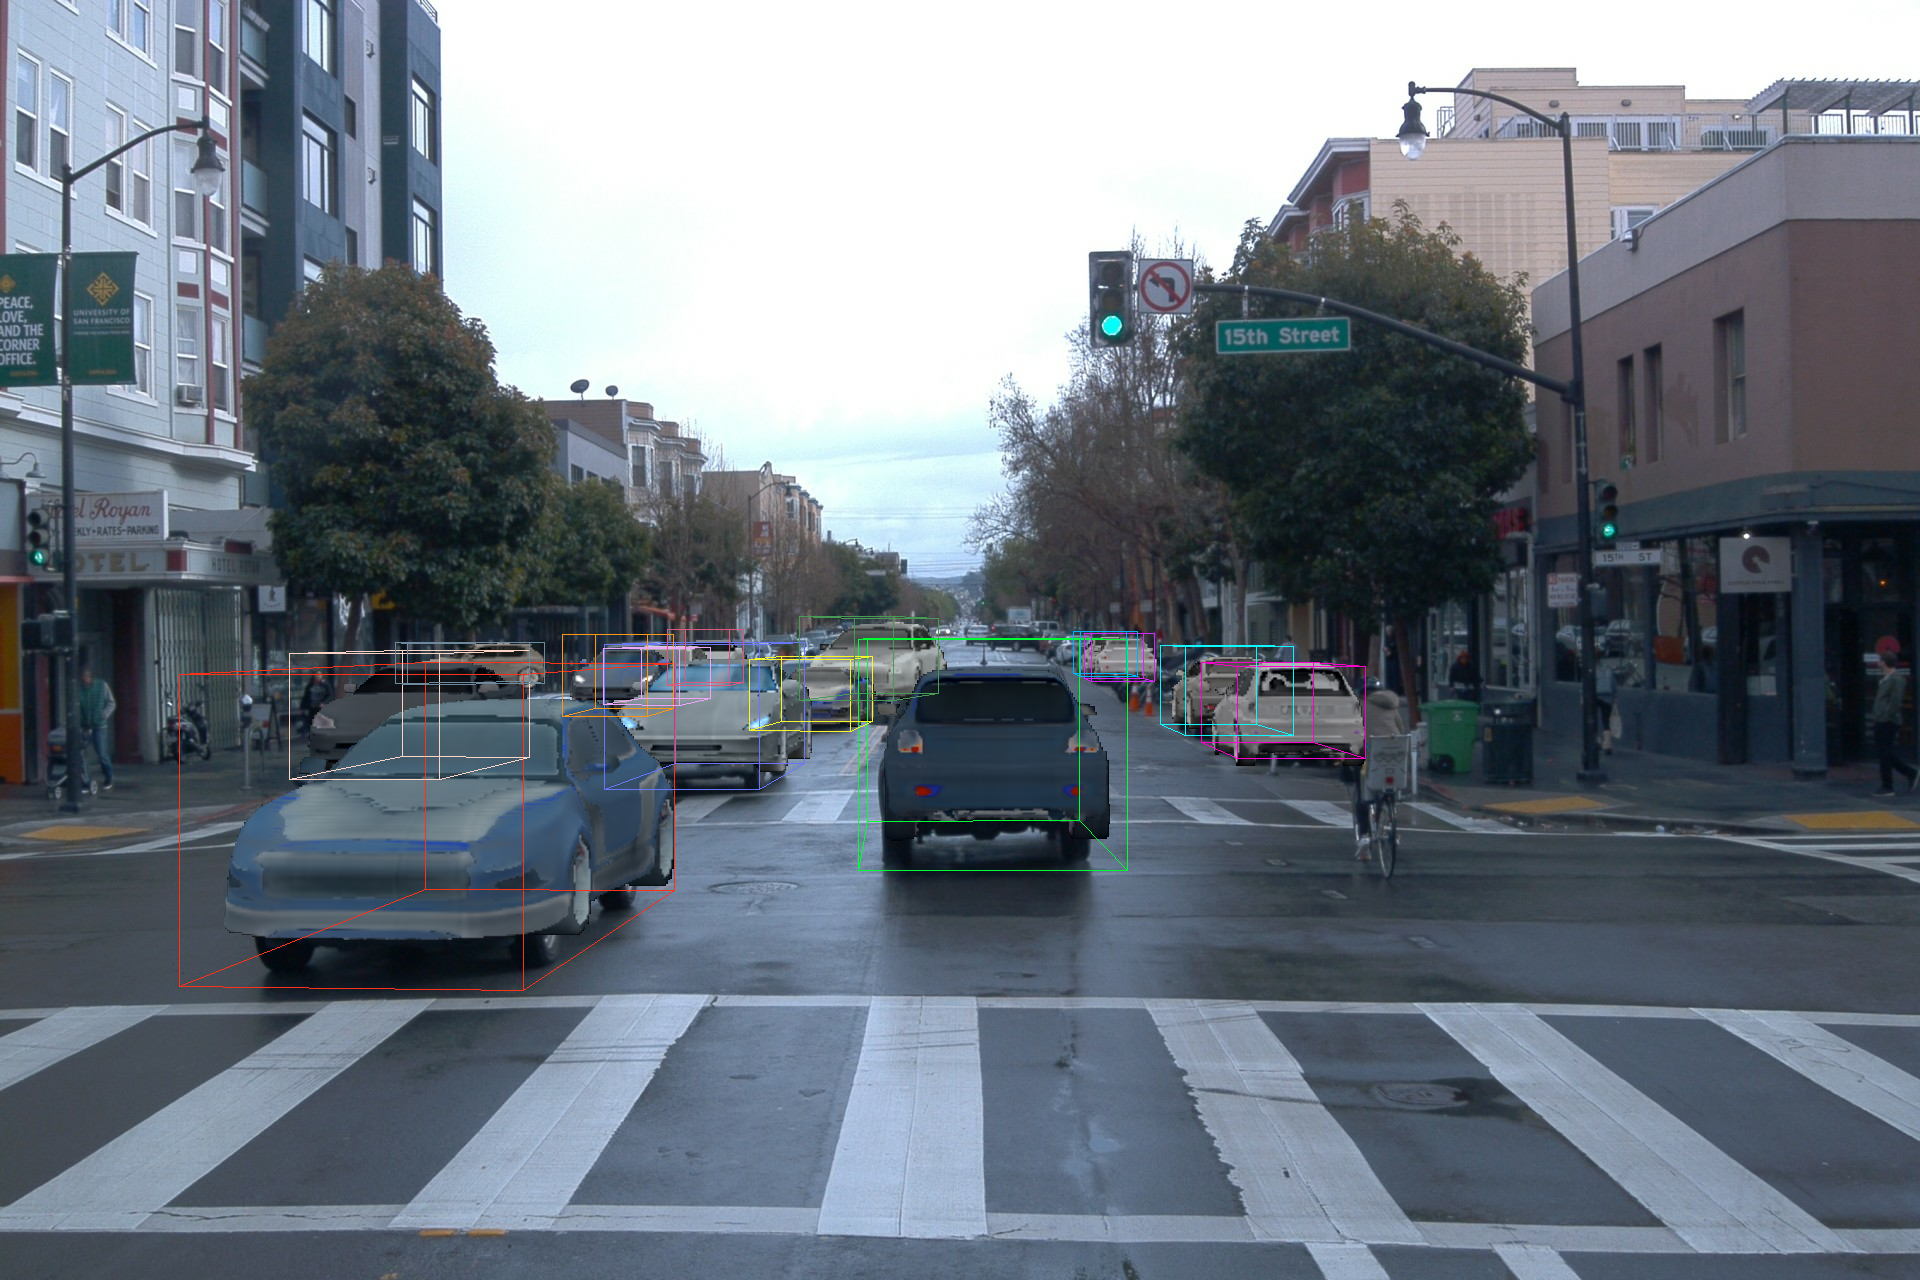
\includegraphics[width=.32\columnwidth, trim={0cm 0cm 0cm 0cm},clip]{fig/waymo_main/scene2/waymo_44_41_bbox.png}}\\%[0.0cm]
		
		
	\end{tabular}
	}
\vspace{-6pt}
\caption{Without changing the model or training on the dataset, our proposed method can generalize well to the Waymo Open Driving Dataset ~\cite{sun2020scalability}. Similar to Fig \ref{fig:nuScenes_results}, from left to right, we show (i) observed images from diverse scenes from the dataset at timestep $k=0$; (ii) an overlay of the closest generated object and predicted 3D bounding boxes at timestep $k=0, 1, 2 \text{ and } 3$. The color of the bounding boxes for each object corresponds to the predicted tracklet ID. Our method does not lose any tracks even on a different unseen dataset in diverse scenes, validating that the approach generalizes.}\label{fig:waymo_results}
\vspace*{-14pt}
\end{figure*}

% We first show the initial input frame at timestep k=0. Next to it, we present an overlay of the closest generated object and the refined bounding boxes. Reconstructions and bounding boxes for the next 3 frames are presented next to it. \todo{Description. Talk about color coding and that you don't lose any detections.}